\documentclass[11pt,a4paper]{jsarticle}

\usepackage[dvipdfmx]{graphicx}
\usepackage{fancyvrb}
\usepackage{ascmac}
\usepackage{mediabb}

\begin{document}

\title{並列分散処理 最終報告書}
\author{135772H 上原可意\\145758G 森井大介\\155702F 大城由也\\155728K 津嘉山遼\\155737J 松本直也\\}
\date{2017/8/2}

\maketitle
\newpage
\section*{目的}
ソートの並列化を行うことにより様々なファイル、名簿などのソートを高速に行うことができる。これにより全てのファイル名をアルファベット順に参照する際などに、PCが素早く対応でき、快適に使用することが可能になる。

\section*{演習の背景}
私たちの班は当初、入力された文字列を受け取り一つずつランダムにシャッフルし、その文字をマージソートでソートするという内容の実験を行うつもりであった。実際にはランダムにシャッフルする部分までは実装できたが、その文字列をシャッフルする際NULLまで受け取ってシャッフルしてしまう問題が発生。期日までに並列化に着手できないと判断し、入力を受け取るパターンからランダムに文字列を生成するパターンに切り替えた。

\section*{方法}
今回は数字をランダムに生成しそのランダムに生成された数字をマージソートで並び替えるという内容である。ソースpp\_marge.cはマージソートを並列処理で処理を行うプログラムである。non\_pp\_marge.cは逐次処理でマージソートが行われるプログラムである。演習の背景の部分にもある通りもともとの内容としては文字列のマージソートを行う予定であった部分でできたところまでを以下に示す。内容としては入力した文字列を配列化し入力した文字列の配列をランダムに並べ替えてそれをマージソートするプログラムを逐次処理と並列処理で処理時間を比較するという方針だった。だが実際は、数字のマージソートができてはいたが文字列の配列をランダムに入れ替えるところまでの実装になった。

\begin{figure}[htbp]
 \begin{tabular}{c}
  \begin{minipage}{0.5\hsize}
   \begin{center}
   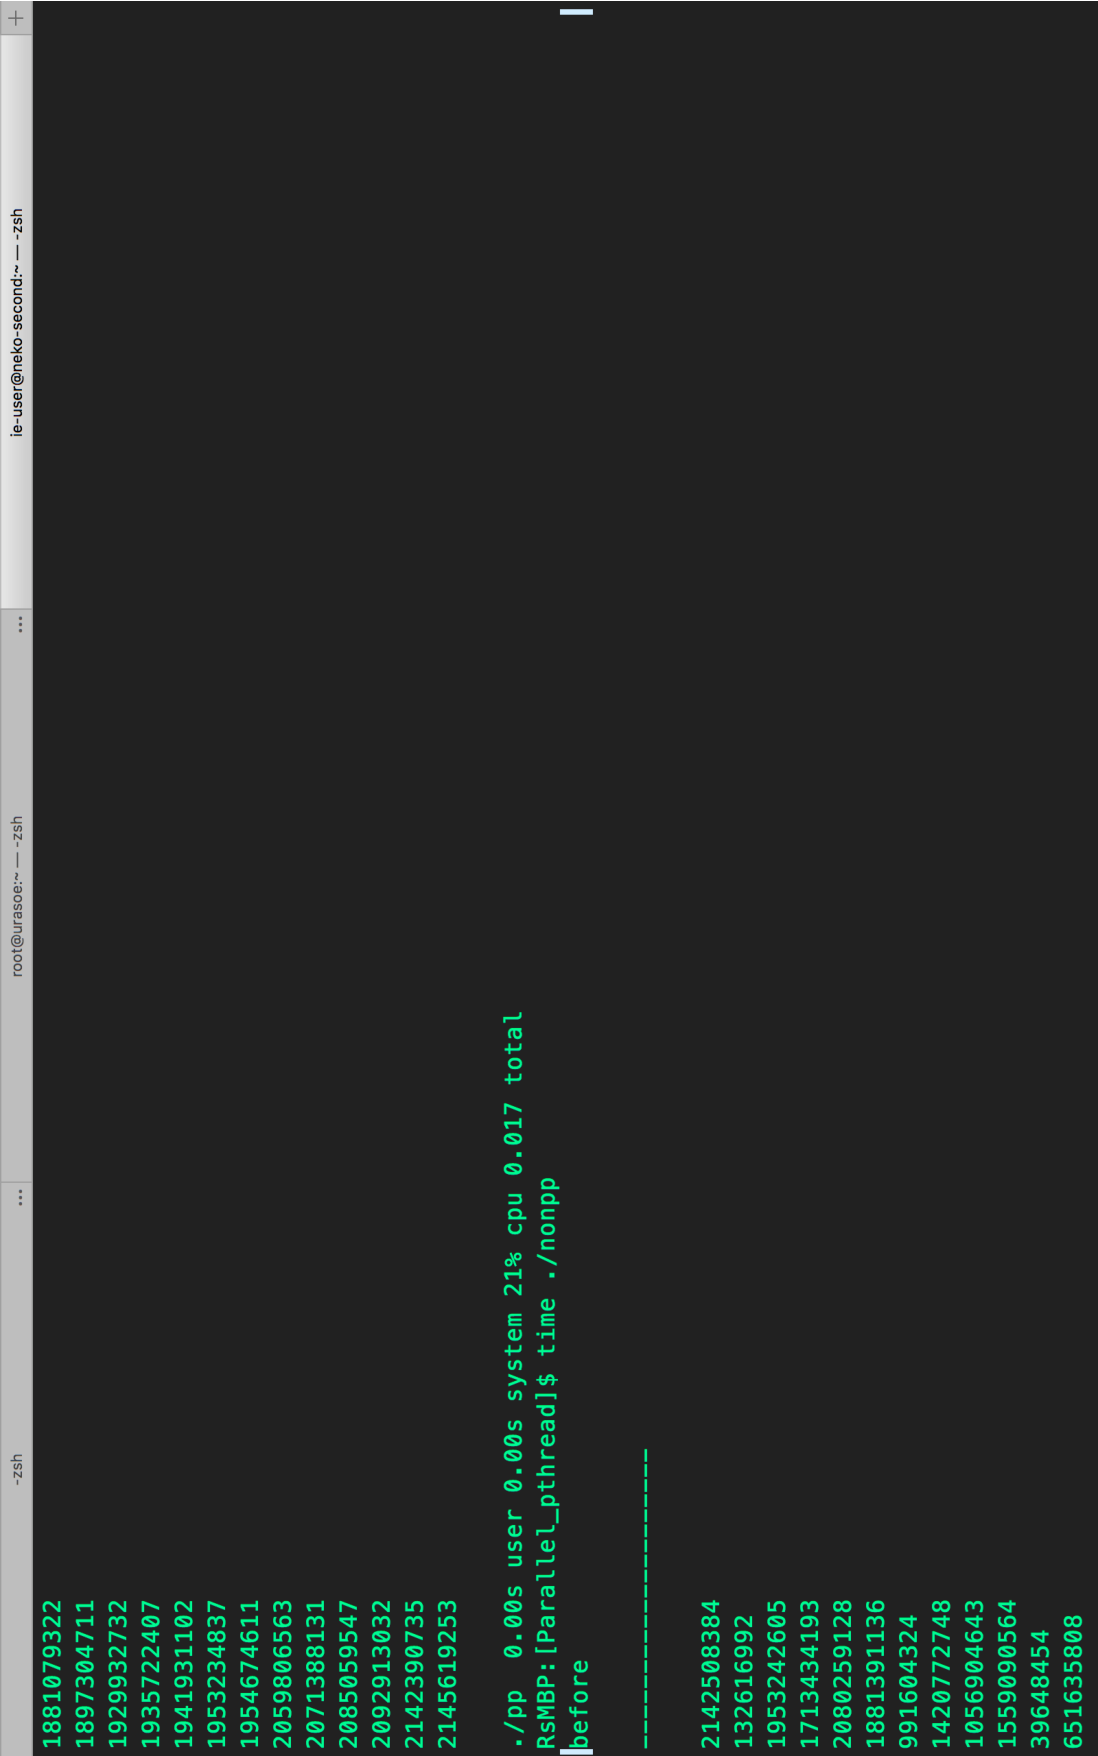
\includegraphics[width=8cm,height=12cm,angle=270]{image2-crop.pdf}
   \caption{並列化したマージソートの実行結果}
   \end{center}
  \end{minipage}
 \end{tabular}
\end{figure}
\begin{figure}[htbp]
 \begin{tabular}{c}
  \begin{minipage}{0.5\hsize}
   \begin{center}
   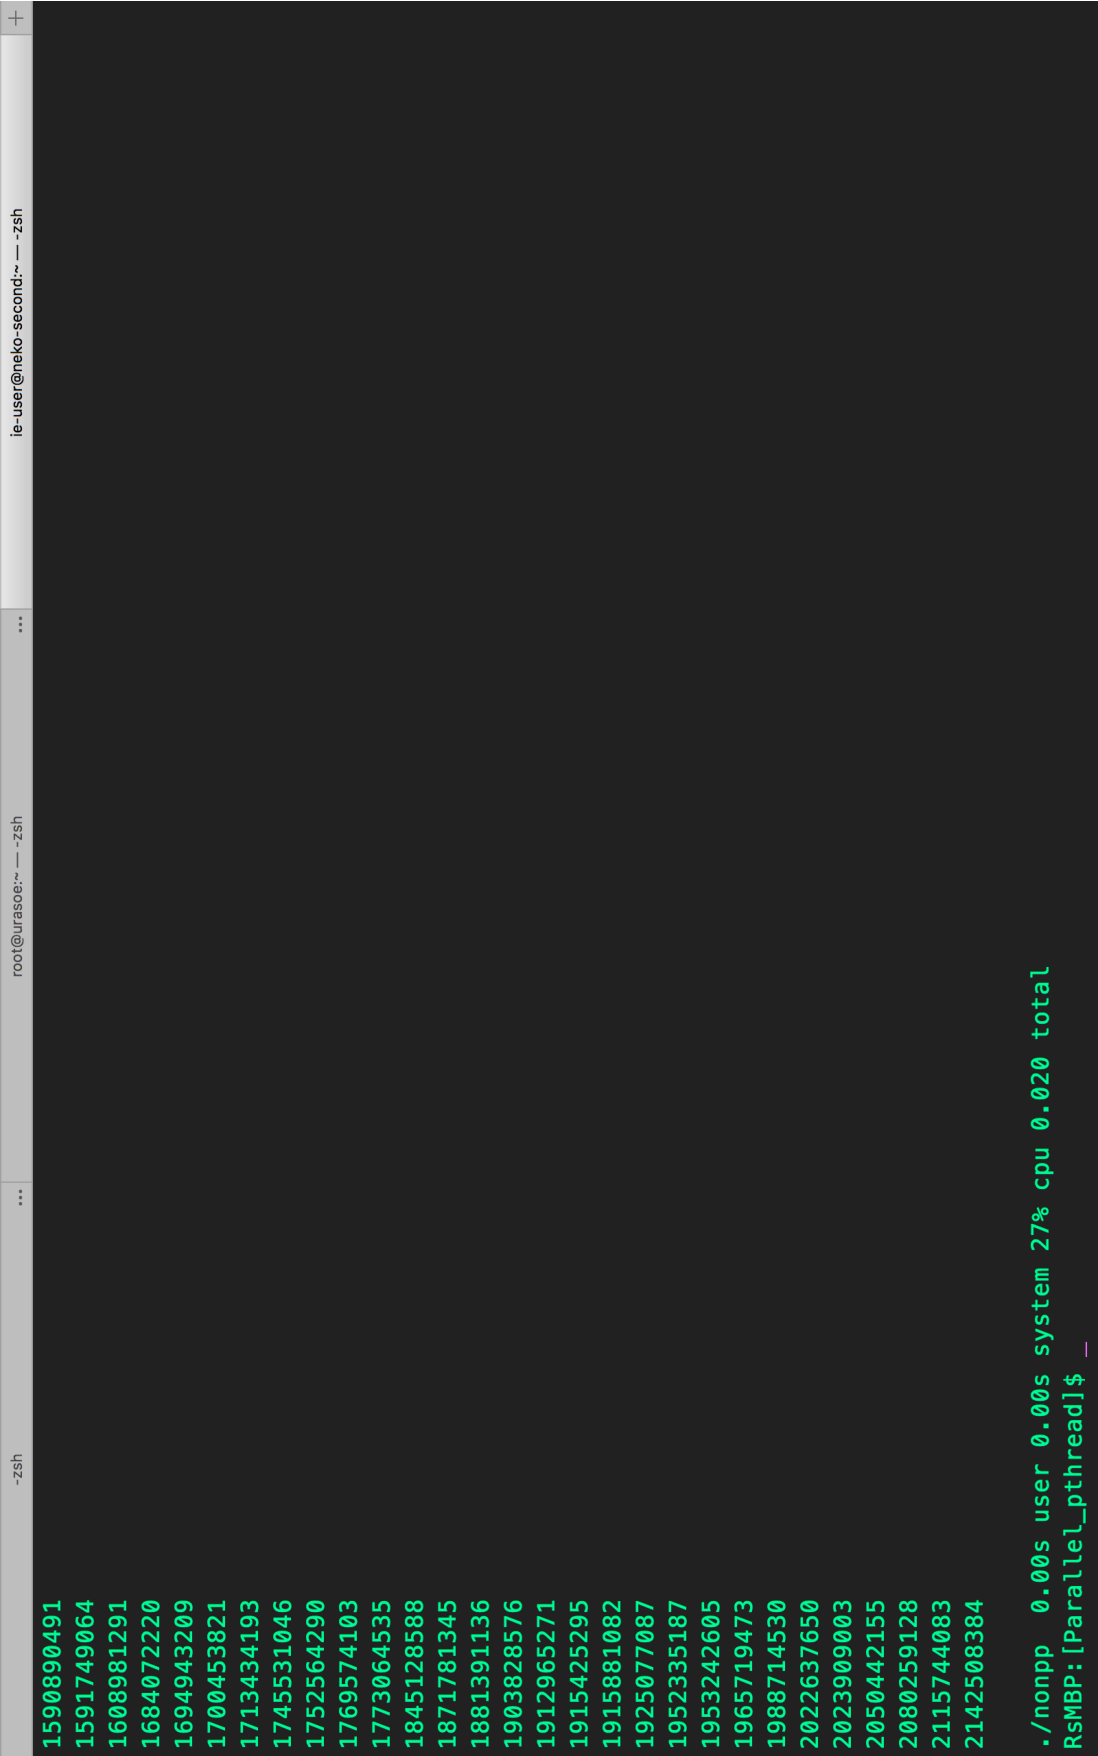
\includegraphics[width=8cm,height=12cm,angle=270]{image3-crop.pdf}
   \caption{逐次処理のマージソート実行結果}
   \end{center}
  \end{minipage}
 \end{tabular}
\end{figure}

\newpage
\begin{figure}[htbp]
 \begin{tabular}{c}
  \begin{minipage}{0.5\hsize}
   \begin{center}
   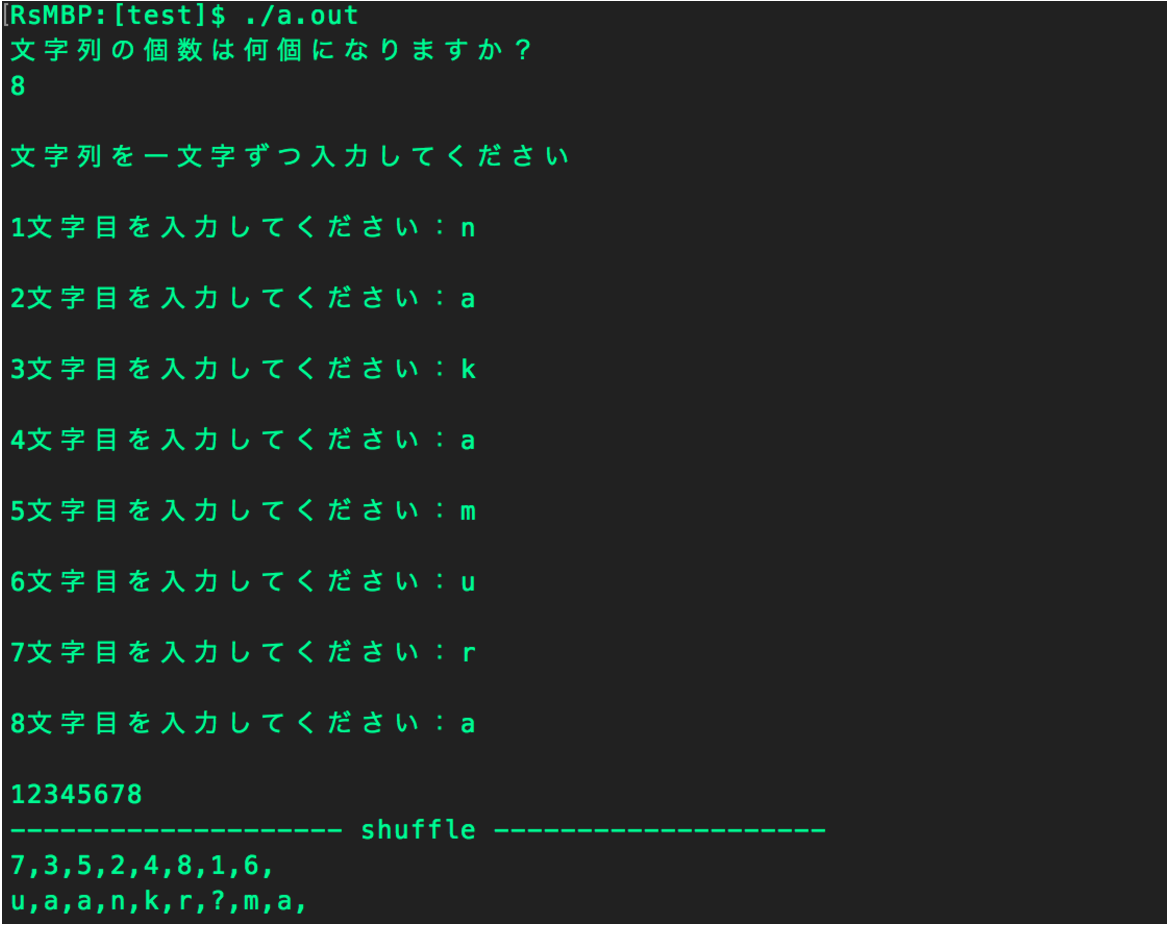
\includegraphics[width=10cm,height=10cm,angle=0]{image4-crop.pdf}
   \caption{実際に仕上げたかったプログラム(NULLまで受け取ってしまっている)}
   \end{center}
  \end{minipage}
 \end{tabular}
\end{figure}

\section*{考察}
今回初期の計画としては文字列を引数として与えてその文字列をランダムな確率でバラバラにしてソートして元の文字列に戻す、という処理を行いたかった。入力された文字列をshuffle関数というその時の時間でランダムに文字列を入れ替える関数を使って文字列をバラバラにした。しかし、C言語と文字列の相性の悪さがここで顕著に現れてきた。NULL文字の扱いや構造体へのデータの格納などと時間の関係上、実装が困難であると判断せざるを得なかった。そこで、ある大きさの数列をランダムに生成して並列化、ソートするという手法に切り替えました。またその際に比較対象として並列化していないソートを用意して比較しました。
また、今回行なっているのが少ない階層のマージソートな上に数列数がそこまで多くないので実行時間に大きな変化は見られなかったが、これがマージソートの階層と数列数が多くなっていくと比例的に実行時間に大きな差がでてくるものと考察できる。


\end{document}